\documentclass[10pt]{beamer}
\usetheme{metropolis}  
\usecolortheme{lily}
\usepackage{hyperref}
\usepackage{bigints}
\usepackage{verbatim}
\title{Introducci\'on a la probabilidad y estad\'istica CM274}
 \usepackage[spanish]{babel}
\date{\today}
\author{C\'esar Lara Avila}
\institute{\url{https://github.com/C-Lara}}
\begin{document}
  \maketitle
  \section{2. Combinatoria para probabilidad }
  
\begin{frame}{Introducci\'on}
Existen muchas t\'ecnicas, basadas en la ley de probabilidad total para contar todas las posibilidades. Es usual describir este problema en t\'erminos de c\'omo se pueden elegir \texttt{bolas distinguibles} de una caja  asumiendo que la elecci\'on es \texttt{aleatoria}, es decir, cada bola en la caja es igualmente probable que se elija.

\vspace{0.2cm}

Alternativamente, el problema puede ser expresado en t\'erminos de c\'omo se pueden insertar \texttt{bolas indistinguibles} en cajas distinguibles. 

\vspace{0.2cm}

Esta primera forma  se llama \textbf{problema de selecci\'on}  y la  \'ultima forma  se llama \textbf{problema de asignaci\'on}. Formularemos nuestra notas en t\'erminos del problema de selecci\'on.
\end{frame}
  
 \begin{frame}{Principio del conteo}
 	
Las t\'ecnicas de conteo consideradas en un espacio muestral con puntos igualmente probables  se basan en dos principios de conteo fundamentales relativos a  eventos mutuamente exclusivos $A$ y $B$:

\vspace{0.2cm}

 \begin{itemize}
 	\item \texttt{Principio 1:} Si los eventos $A$ y $B$ pueden ocurrir en $n$  y $m$ maneras respectivamente, entonces $A$ y $B$ pueden ocurrir juntos de $nm$ maneras, llamada \textcolor{orange}{regla de multiplicaci\'on}.
 	\item \texttt{Principio 2:} Si los eventos $A$ y $B$ pueden ocurrir en $n$  y $m$ maneras respectivamente, entonces $A$ o $B$ pueden ocurrir juntos de $n + m$ maneras, llamada \textcolor{orange}{regla de suma}.
 \end{itemize}


\end{frame}
\begin{frame}{Principio del conteo(1)}
El Principio $1$ se establece f\'acilmente ya que $A$ puede ocurrir de $n$ maneras y luego debe ser seguida por cada manera  en que $B$ puede ocurrir. Un diagrama de \'arbol, mostrado en la siguiente figura ilustra el resultado.

 \begin{figure}[h]
 	\centering
 	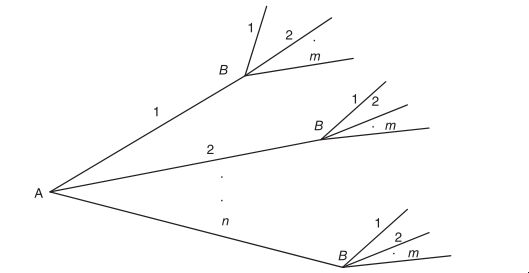
\includegraphics[width=7cm]{c1}
 \end{figure}
 
 \vspace{0.2cm}
 
El Principio $2$ simplemente usa la palabra \texttt{o} en un sentido exclusivo.

\end{frame}

\begin{frame}{Permutaciones}
Una disposici\'on (arreglo ) de \'items, tambi\'en llamada una \underline{\texttt{secuencia ordenada} de \'items }, se dice que es una permutaci\'on de los \'items. Una secuencia ordenada de $n$ \'items  se llama una \underline{$n$-permutaci\'on}.



Con $n$ \'items  distintos, hay \textcolor{blue}{$n!$} permutaciones posibles. Este es el n\'umero de diferentes maneras en que los n \'items distintos pueden ser colocados, ordenados

\vspace{0.3cm}

\small{

\textbf{Ejemplo}

\vspace{0.2cm}
	
Considera la palabra PUPPY. Si los cinco caracteres fueran distintos, el n\'umero de permutaciones que se obtendr\'ia seria $5!$. Sin embargo, como el car\'acter P aparece tres veces en PUPPY, el $5!$ debe ser dividido por $3!$, para obtener $5!/3! = 5\times  4 = 20$. El n\'umero de diferentes maneras en que los caracteres de la palabra PUPPY se pueden colocar o disponer  es por lo tanto $20$.}

\end{frame}

\begin{frame}{Permutaciones con reemplazo}
En el caso de permutaciones con reemplazo, nuestro objetivo es contar el n\'umero de formas en que se pueden seleccionar $k$ bolas entre $n$ bolas distinguibles. Despu\'es de cada bola es elegida y sus caracter\'isticas son registradas, se sustituye en la caja y se elige la bola siguiente.

\vspace{0.2cm}

Si $k = 1$(se elige una bola), entonces el n\'umero de permutaciones posibles es $n$, ya que cualquiera de las $n$ bolas puede ser elegida. Si $k = 2$, entonces cualquiera de las $n$ bolas puede ser elegida como la primera bola y luego reemplazada en la caja. Para cada una de estas $n$ elecciones de la  primera bola, la siguiente bola elegida puede ser tambi\'en cualquiera de las $n$ bolas distinguibles y por lo tanto el n\'umero de permutaciones cuando $k = 2$ es $n\times n = n^2$.

\vspace{0.2cm}

Este razonamiento puede continuar y  demostrar que el n\'umero de permutaciones obtenidas para cualquier \textcolor{red}{$k$ es $n^k$}.

\end{frame}

\begin{frame}{Permutaciones con reemplazo(1)}
Supongamos ahora que hay $n_1$ maneras de elegir un primer elemento (\'item ) y $n_2$ formas de elegir un segundo elemento(\'item). Entonces el n\'umero de pares ordenados distintos es igual a $n_1n_2$. 


En t\'erminos de bolas distinguibles en cajas, esto puede ser visto como el n\'umero de maneras en que una bola puede ser elegida de una primera caja que contiene $n_1$ bolas distinguibles y una segunda bola elegida de una segunda caja que contiene $n_2$ bolas distinguibles.  


Si hay $n_i$ formas de elegir un \'item i, para $i = 1,2,\dots, k$ , entonces el n\'umero de k-tuplas ordenadas distintas es igual a \textcolor{orange}{ $n_1n_2\dots n_k$}.

\vspace{0.2cm}

\small{
	
	\textbf{Ejemplo}
	
	El n\'umero de c\'odigos de cuatro d\'igitos que se pueden obtener utilizando el sistema de n\'umeros decimales (con diez d\'igitos de $0$ a $9$ inclusive) es $10^4 = 10.000$. Estos son los c\'odigos que van desde $0000$ hasta $9999$.
}

\end{frame}

\begin{frame}{Permutaciones sin  reemplazo}
Pasemos ahora al problema de contar el n\'umero de diferentes permutaciones obtenidas al seleccionar $k$ bolas de entre $n$ bolas distinguibles en el caso de que una vez que se elija una bola en  particular, esta  no se devuelve a la caja.
	
Denotamos a este n\'umero como  $P(n, k)$ y asignamos los valores $P(n, 0) = 1, n = 0,1,\dots $, por convenci\'on.

Decimos que $P(n, k)$ es el \underline{n\'umero de permutaciones} de $n$ objetos tomados $k$ a la vez.
	
\vspace{0.2cm}
	
\small{Si $k = 1$, entonces cualquier bola puede ser elegida y el n\'umero total de permutaciones  simplemente es  $n$. Si $k = 2$, entonces cualquiera de las $n$ bolas puede ser elegida como la primera, para cada una de estas $n$ elecciones posibles, quedan $n - 1$ bolas en la caja, cualquiera de las cuales puede ser elegida como la segunda. As\'i, el n\'umero total de permutaciones para $k = 2$ es igual a $n (n - 1)$.}
\end{frame}

\begin{frame}{Permutaciones sin  reemplazo(1)}

\small{Con $k = 3$, hay $n$ posibilidades diferentes para la primera bola,  $n-1$ para la  segunda y $n-2$ para la  tercero, lo que da $P (n, 3) = n (n -1) (n -2 )$.
 
Podemos ahora generalizar esto a cualquier arbitrario $k \leq n $ para obtener
 
 \[
 P(n,k) = n(n - 1)(n - 2)\dots(n - k + 1) =\frac{n!}{(n - k)!}.
 \]
}

\small{

Sea $n = 4, k = 3$ y distinguimos las cuatro bolas por medio de las  letras A, B, C y  D. Tenemos $P(4,3) = 4 \times 3 \times 2 = 24$. Esas 24 posibilidades, est\'an dadas por:


\qquad \qquad \qquad \qquad \texttt{ABC, ABD, ACB, ACD, ADB, ADC,}

\qquad \qquad \qquad \qquad \texttt{BAC, BAD, BCA, BCD, BDA, BDC,}

\qquad \qquad \qquad \qquad \texttt{CAB, CAD, CBA, CBD, CDA, CDB,}

\qquad \qquad \qquad \qquad \texttt{DAB, DAC, DBA, DBC, DCA, DCB.}
}

\vspace{0.2cm}

\scriptsize{Debes observar  que distinguimos entre  ABC y ACB, ya que el orden es importante, pero no incluimos la misma letra m\'as de una vez (por ejemplo, AAB no est\'a presente), esto es por  que una vez  que las letras son usadas no pueden ser utilizadas de nuevo.}
\end{frame}

\begin{frame}{Combinaciones sin reemplazo}
Sea al caso en el que las bolas se seleccionan sin reemplazo, pero el orden en que se seleccionan no tiene importancia. Lo \'unico que importa es que se han elegido algunas bolas y la forma en  que se seleccionaron  no es de inter\'es.

Por ejemplo, podemos haber elegido una bola verde, una bola roja y una bola negra, pero  no sabemos o no nos preocupamos cu\'al de estas tres fue elegida primera, segunda o tercera. 

\vspace{0.2cm}

Sea  \textcolor{orange}{$C(n, k)$} que  denota  el n\'umero de maneras en que se pueden seleccionar $k$ bolas sin reemplazo e independientemente de su orden en  una caja que contiene $n$ bolas. Este s\'imbolo se dice que es el n\'umero de combinaciones de $n$ elementos tomados $k$ a la vez,  no teniendo en cuenta el orden.

\end{frame}

\begin{frame}{Combinaciones sin reemplazo(1)}
Dado que cualquier secuencia de $k$ \'items puede ser dispuesta  en $k!$ permutaciones, se deduce que debe haber $k!$ veces m\'as permutaciones (sin reemplazo) de $k$ \'items  distintos de lo que hay en  combinaciones (sin reemplazo), ya que el orden  importa en permutaciones, pero no en combinaciones. En otras palabras, debemos tener

\[
k!C(n,k) = P(n,k) \ \ \text{para}\ \   n = 0,1,2,\dots \ \ \text{y}\ \  k = 0,1,\dots, n.
\]


Esto conduce al siguiente resultado conocido: 

\[
C(n, k) = \frac{P(n ,k)}{k!} = \frac{n!}{k!(n -k)!}\ \ \text{para}\ \ n = 0, 1, 2, \dots \ \ \text{y}\ \ k = 0,1,\dots, n.
\]

\end{frame}

\begin{frame}{Combinaciones sin reemplazo(2)}

\small{Sean A, B, C, D y E cinco elementos distinguibles de los cuales dos deben ser escogidos (lo cual implica, sin reemplazo, y no importa cu\'al viene primero: es decir, una combinaci\'on). El n\'umero de formas en que estos dos pueden ser elegidos est\'a dado por $C(5,2) = 5!/(2!3!) = 10$. Estos son los resultados:


\qquad \qquad \texttt{AB    AC   AD   AE}

\qquad \qquad \texttt{BC   BD   BE}

\qquad \qquad  \texttt{CD   CE}

\qquad \qquad  \texttt{DE}
}

\vspace{0.2cm}


$C(n, k)$ se denomina \underline{coeficiente binomial} ya que  es el coeficiente del t\'ermino $p^k q^{n-k}$ en la expansi\'on del binomio $(p + q)^n$. Formas alternativas para escribir este coeficiente binomial son:

\[
C(n , k) = C_{k}^{n} = \binom{n}{k}.
\]

\end{frame}
\begin{frame}{Combinaciones sin reemplazo(3)}

\small{Para calcular los coeficientes binomiales, notamos que

\begin{align*}
\binom{n}{k} & = \frac{n!}{k!(n - k)!} = \frac{n}{k}\Biggl(\frac{(n -1)!}{(k -1)!(n -k)!} \Biggr)\\
& = \frac{n}{k}\Biggl(\frac{(n -1)!}{(k -1)!([n -1] -[k -1])!}\Biggr) = \frac{n}{k}\binom{n - 1}{k -1}
\end{align*}


Lo que conduce a, 



\[
\binom{n}{k} = \frac{n}{k}\times\frac{n -1}{k -1}\times \cdots \times \frac{n - (k -1)}{k - (k -1)} = \displaystyle \prod_{j =1}^{k}\frac{n - j + 1}{j}.
\]



y esta expresi\'on  computacionalmente es m\'as eficiente   que formar factoriales y tomar razones}.

\end{frame}
\begin{frame}{Ejemplo explicativo}
Consideremos ahora el problema de colocar $k$ bolas distinguibles en $n$ cajas diferentes de tal manera que el n\'umero de bolas en la caja $i$ sea $k_i$ para $i = 1,2, \dots, n$.

\vspace{0.2cm}

Asumimos que $\displaystyle \sum_{i =1}^n k_i = k$ , de modo que cada bola se pone en una de las cajas y de manera que no queda ninguna.


\vspace{0.2cm}

El n\'umero de combinaciones obtenidas al seleccionar las primeras $k_1$ bolas para la caja 1 es $C(k, k_1)$. Esto deja  $k -k_1$ bolas, de las cuales $k_2$ son escogidas y colocadas en la caja 2. El n\'umero de combinaciones obtenidas al seleccionar estas $k_2$ bolas  de las  $k - k_1$ bolas es $C(k- k_1, k_2)$, de modo que el total obtenido de las  dos primeras cajas es $C(k, k_1)\times C(k - k_1, k_2)$.

\end{frame}
\begin{frame}{Ejemplo explicativo(1)}
\small{Continuando de esta manera, vemos que el n\'umero total de combinaciones est\'a dado por:

\[
C(k, k_1)\times C(k -k_1, k_2) \times C(k -k_1 - k_2, k_3)\times \cdots \times C\Biggl( k - \sum_{i =1}^{n -1}k_i, k_n\Biggr),
\]



donde $ C( k - \sum_{i =1}^{n -1}k_i, k_n) = C(k_n, k_n)$. Sustituyendo en la f\'ormula para los n\'umeros de combinaci\'on tenemos:

\begin{align*}
\frac{k!}{k_1!( k - k_1)!} \times \frac{(k -k_1)!}{k_2!( k - k_1 -k_2)!} \times  \frac{(k -k_1 -k_2)!}{k_2!( k - k_1 -k_2 - k_3)!}\times \cdots \\
=\frac{k!}{k_1!k_2!\cdots k_n!}\equiv \binom{k}{k_1, k_2,\dots k_n}.
\end{align*}

\vspace{0.2cm}

Estos son los llamados \underline{coeficientes multinomiales}.
}
\end{frame}
\begin{frame}{Combinaciones con reemplazo }
	
\small{Cuando se seleccionan $k$ bolas con reemplazo de una caja que contiene $n$ bolas distinguibles. Se puede demostrar que esto es id\'entico al problema de contar el n\'umero de combinaciones cuando se seleccionan $k$ bolas sin sustituci\'on de una caja que contiene un total de $n + k- 1$ bolas distinguibles, es decir:
	
	\[
	\frac{(n + k -1)!}{(n -1)!k!}.
	\]

\vspace{0.2cm}

Representamos las $n$ bolas por estrellas adyacentes y consideramos la posibilidad de insertar $k -1$ barras entre las estrellas para separar las barras en $k$ en grupos. Por ejemplo, para $n =12$ y $k =5$, la siguiente es una representaci\'on de un grupo  de $12$ bolas indistinguibles en $5$ urnas, donde el tama\~no de las urnas $1$, $2$, $3$, $4$ y $5$ son $2$, $4$, $0$, $3$ y $3$, respectivamente:

\vspace{0.2cm}

\begin{figure}[h]
	\centering
	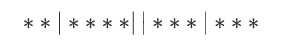
\includegraphics[width=5cm]{c2}
\end{figure}
	}
\end{frame}

\begin{frame}{Combinaciones con reemplazo(1)}
	
Se debe tener  en cuenta que en la agrupaci\'on,  pueden haber urnas vac\'ias. Hay un total de $n + k -1$ posiciones, de las cuales $n$ son estrellas y $k -1$ son barras. Por lo tanto, el n\'umero de formas de colocar $n$ bolas indistinguibles en $k$ urnas etiquetadas es el mismo que el n\'umero de formas de escoger $n$ posiciones entre $n -k + 1$ espacios para las estrellas, con todas las posiciones restantes tomadas como barras.

\vspace{0.5cm}

El n\'umero de maneras en que esto se puede hacer es: $\binom{n + k -1}{n}$. Pero	 $\binom{n + k -1}{n} =  \binom{n + k -1}{k -1}$ puede interpretarse como el n\'umero de formas de elegir las posiciones de las barras y tomar todas las posiciones restantes como estrellas.
\end{frame}

\begin{frame}{Ejemplo explicativo}
	
Veamos el caso que  $n = 4$  y diferenciamos las bolas con las letras  A, B, C y D. Si elegimos k = 3 entonces la f\'ormula nos dice que hay $(4+ 3- 1)!/(3! \times 3!) = 20$ combinaciones diferentes. Estas son:



\qquad \qquad \texttt{AAA   AAB   AAC   AAD  ABB  ABC  ABD   ACC  ACD   ADD}

\qquad \qquad \texttt{BBB  BBC  BBD   BCC  BCD   BDD}

\qquad \qquad \texttt{CCC  CCD   CDD}

\qquad \qquad \texttt{DDD}.


\vspace{0.2cm}

\small{Debes de observar  que, aunque las cuatro bolas se distinguen, la misma bola puede aparecer m\'as de una vez en una combinaci\'on dada. Esto se debe a que despu\'es de que una bola ha sido elegida, esta  se sustituye y se puede elegir una vez m\'as.
	
 Observa  tambi\'en que no incluimos combinaciones como BAA o CBA porque con combinaciones, el orden no es importante y estas son equivalentes a AAB y ABC, respectivamente.}
\end{frame}
\end{document}